\section{Evaluation}
\label{sec:eval}

\subsection{What we measured, and where}
\label{sec:eval:testbed}

\textbf{Evaluation Cases.} We compare two arms of the same program, differing only in the release
schedule. In \emph{Timing OFF} the switch forwards the outstation's acknowledgment and response as
they arrive; in \emph{Obfuscated} it holds them and releases them on the deadlines of
Section~\ref{sec:design}. The switch is the only path between the master and the relay, and every
timestamp is taken on the master-facing link, so each interval below is one a passive observer can
record: the arrival of the transport acknowledgment to the arrival of the application response,
both on the master's own interface. The switch's internal instants are on links that were not
captured and are recovered from the program rather than measured.

\textbf{Configuration provenance is partial.} Each block's manifest records the policy it was
configured with and the loaded program's identity, but the sweep has no per-point readback of what
the device held. Every policy value in this section is the configured one unless we say otherwise,
and we mark where a readback would have settled a question the configuration cannot.

\textbf{Dataset.} We report per DNP3 exchange. The campaign holds 63{,}360 of them, half with the
mechanism running and half without, collected over five hours in interleaved blocks so that drift
cannot separate the two arms. Every request was answered, and no exchange was retransmitted,
malformed or excluded. A separate sweep on the same testbed covers 16 configured policies and
three controls with the mechanism disabled.

\subsection{Does the released interval reach its configured value? (RO1)}
\label{sec:eval:ro1}

\begin{figure}[tbp]
  \centering
  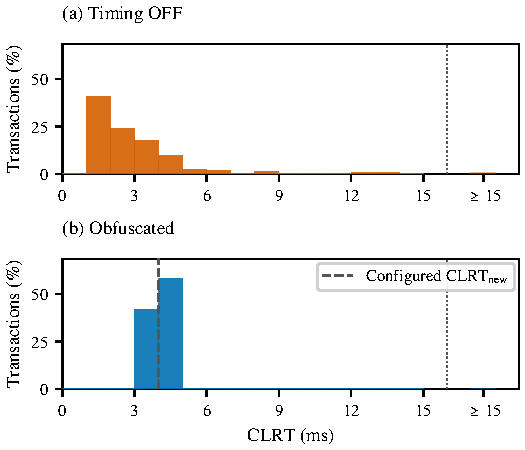
\includegraphics{figures/clrt/fig_clrt_distributions}
  \caption{Measured READ CLRT before and after obfuscation, as the percentage of each arm's own
  transactions per bin, on common 1~ms bins anchored at 0~ms with a linear ordinate. Finite bins
  are half-open; the hatched category holds everything at or above 15~ms, 0.409\% of (a) and
  0.027\% of (b). The dashed line in (b) is the configured $\mathrm{CLRT}_{\mathrm{new}}$, which
  falls on a bin edge, so the obfuscated mass divides between the two neighbouring bins;
  Figure~\ref{fig:clrtzoom} resolves it. In (a) $n$~=~26{,}400, mean 2.800~ms, sd 2.609~ms,
  variance 6.808~ms$^2$; in (b) $n$~=~26{,}400, mean 4.012~ms, sd 0.628~ms, variance
  0.394~ms$^2$.}
  \label{fig:hist}
\end{figure}

\begin{figure}[tbp]
  \centering
  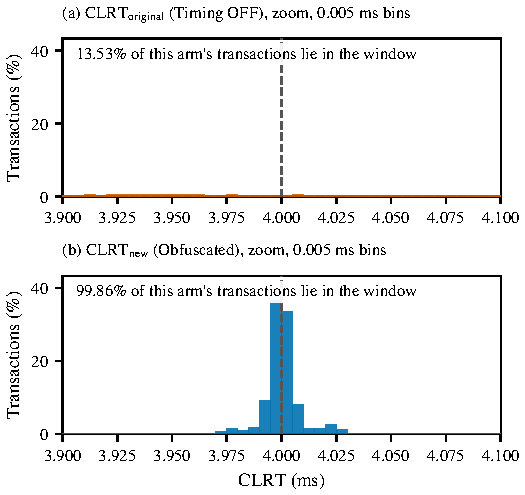
\includegraphics{figures/clrt/fig_clrt_zoom}
  \caption{The released interval, resolved. The same measurements as Figure~\ref{fig:hist} on
  0.005~ms bins within $0.10$~ms of the configured $\mathrm{CLRT}_{\mathrm{new}}$ (dashed). The
  ordinate is still the percentage of that arm's entire sample, not of the window, so the bars
  are directly comparable with the other figures. The window holds 13.58\% of (a) and 99.86\% of
  (b).}
  \label{fig:clrtzoom}
\end{figure}

\textbf{RO1.} The read-path schedule of~(\ref{eq:schedule}) does replace
$\mathrm{CLRT}_{\mathrm{original}}$ with the configured $\mathrm{CLRT}_{\mathrm{new}}$. We compare
the two arms over all 22 grouped runs as full empirical distributions, because the shape of the
Timing OFF distribution is what makes a single observation informative to an adversary.

Figure~\ref{fig:hist} shows the two READ distributions. Before obfuscation the interval is broad
and multi-modal, spanning 1.01 to 83.46~ms with peaks near 1.2, 2.1 and 4.0~ms; after it, 99.9\% of
transactions fall within 0.10~ms of the configured $\mathrm{CLRT}_{\mathrm{new}}$. In
Figure~\ref{fig:clrtzoom} the released interval resolves into a narrow distribution about that
value, where the Timing OFF arm places only 13.6\% of its transactions.

The change is a replacement, not a shift. The standard deviation falls from 2.609 to 0.628~ms for
READ and from 2.267 to 0.024~ms for SELECT, variance ratios of 0.058 (95\% CI [0.019, 0.101]) and
0.0001 (95\% CI [1.4$\times$10$^{-5}$, 3.4$\times$10$^{-4}$]) under a session-level bootstrap. A
defense that shifted the interval would keep that spread, because translating a sample leaves its
variance unchanged: translated onto the protected median, the Timing OFF distribution retains
standard deviations of 2.609 and 2.267~ms, four and ninety-four times what we measure. That
counterfactual is analytical, computed from the Timing OFF samples themselves; the loaded program
has no shifting mode, so it is not a measured arm and we do not present it as one.

Low spread at the wrong interval would not be normalization, so we also report where it sits.
The median $\mathrm{CLRT}_{\mathrm{original}}$ is
2.116~ms for READ and 2.050~ms for SELECT, with interquartile ranges of 2.778 and 2.697~ms; under
the mechanism both medians are the configured 4.000~ms and each interquartile range falls to
0.006~ms, two orders of magnitude below the 1~ms step between neighbouring policy settings in the
sweep of Section~\ref{sec:eval:policy}. The median alone understates the change, because the
Timing OFF distributions rise in a few discrete steps, so one observation can be informative about
the class, whereas the obfuscated ones are a step at the scheduled release, an instant computed
from the acknowledgment and a fixed offset that no longer depends on how long the device took.
Figure~\ref{fig:hist} shows that for READ; the per-class distributions for all three, and the
per-run medians in acquisition order, are published with the artifact.

A tail remains, and it is one-sided: the largest obfuscated READ interval is 57.182~ms, and fewer
than one READ exchange in a thousand departs from the scheduled release by more than 1~ms. The
asymmetry follows from the mechanism, because a response reaching the switch after its scheduled
release cannot be moved backwards and leaves as soon as the hold queue serves it. The mechanism
cannot schedule a release before the response exists. Below the configured value the distribution
is not empty either: each release carries its own queueing and service, so their difference falls
either side of the configured interval, which is why the distribution has width at all. Those late
exchanges are the coverage boundary of RO4 seen from the other side, and we count them rather than
hide them.

\textbf{Stability within the Campaign.} The obfuscated median sits at the scheduled release in
every one of the 22 grouped runs and every class, while the Timing OFF medians stay separated, so
the effect is not an artifact of one run or of drift over the five hours. The per-run medians and
interquartile ranges in acquisition order are published with the artifact.

\subsection{Does the control lane behave the same way? (RO2)}
\label{sec:eval:ro2}

\textbf{RO2.} The control-path rule of~(\ref{eq:control}) holds the master-visible
response-to-ACK interval at the policy value. Timed from the request, its observable is
$O = R - A$, in which the internal hold $J$ does not appear, so the read-path budget $D$ does not
apply to it; the switch draws $J$ per transaction from the configured codebook
$\{2, 6, 12\}$~ms. The OPERATE median moves from 2.937~ms under
Timing OFF to 4.000~ms under the mechanism, the interquartile range falls from 2.827 to 0.006~ms,
and the interval stays concentrated at the configured value in every run. That is a result about
the interval the master sees: the relay-facing release at $T_0 + J$ was not observed
(Section~\ref{sec:eval:limits}).

\subsection{What range of settings does the mechanism support? (RO4)}
\label{sec:eval:policy}

\begin{figure}[tbp]
  \centering
  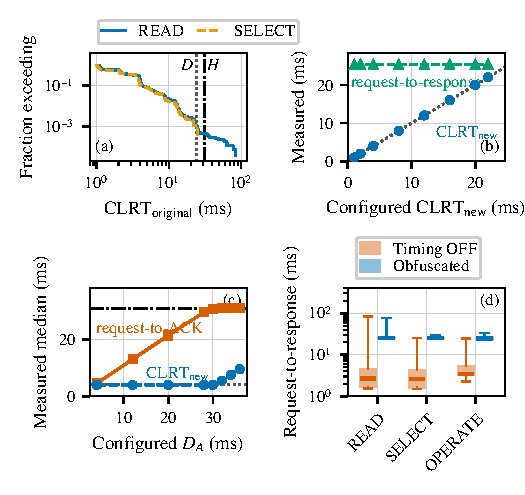
\includegraphics{figures/ndss/fig_policy_coverage_cost}
  \caption{The release policy is programmable and bounded on both sides. (a) Timing OFF read-lane tail
  against the budget $D$ and the horizon $H$. (b) At $D=24$~ms the measured $\mathrm{CLRT}_{\mathrm{new}}$ follows the
  configured $\mathrm{CLRT}_{\mathrm{new}}$ while the response latency stays fixed. (c) Raising $D_A$ saturates near $H$.
  (d) End-to-end response time per class.}
  \label{fig:policy}
\end{figure}

\textbf{RO4.} The interval a passive observer records is a policy value the operator sets, over a
usable range. We installed 16 release policies in turn and ran a fixed DNP3 workload through each,
in two series: the first holds the budget at $D = D_A + \mathrm{CLRT}_{\mathrm{new}} = 24$~ms and
moves the split between them, the second fixes the configured
$\mathrm{CLRT}_{\mathrm{new}}$ at 4~ms and raises $D_A$ until the mechanism leaves its operating
region. Each point is the median over its READ exchanges.

In Figure~\ref{fig:policy}(b) the measured $\mathrm{CLRT}_{\mathrm{new}}$ follows the configured
value along the identity line: settings of 1, 2, 4, 8, 12, 16, 20 and 22~ms give measured medians
of 0.998, 1.999, 3.999, 8.001, 12.001, 16.000, 20.001 and 22.001~ms, while the end-to-end response
time stays between 25.30 and 25.34~ms throughout. The leaking interval and the cost of the
exchange can therefore be set independently, which is what makes the mechanism a framework rather
than one fixed setting. In Figure~\ref{fig:policy}(c) the request-to-acknowledgment interval
tracks $D_A$ up to 30~ms, where the measured median is 30.571~ms and
$\mathrm{CLRT}_{\mathrm{new}}$ still sits at 4.001~ms.

Beyond that the acknowledgment interval saturates at about 31.07~ms and
$\mathrm{CLRT}_{\mathrm{new}}$ can no longer be held, rising to 5.503, 7.498 and 9.507~ms at $D_A$
of 32, 34 and 36~ms, because the reservoir carries a finite pass budget and a hold ends when that
budget is spent. The saturation sits close to the admission horizon $H$, which is what one would
expect if the control plane's assumed service rate is about right, but is not evidence that the
data plane enforces $H$. From below the range is closed by the outstation's own response time,
which the switch cannot anticipate: in Figure~\ref{fig:policy}(a) the 24~ms budget covers
99.900\% of Timing OFF read-lane exchanges, and one in a thousand arrives too late to be held. The
usable range is therefore 1 to 22~ms at a fixed budget.

\subsection{What does the mechanism cost? (RO5)}
\label{sec:eval:cost}

\textbf{RO5.} In Figure~\ref{fig:policy}(d) the median response time rises by 22.7~ms for READ,
22.6~ms for SELECT and 21.2~ms for OPERATE: close to but below the release budget, because it
depends on how long the outstation itself took, and a real operational cost to weigh against the
polling period and any protocol timeout. Each exchange carries 3.017 frames and 272.3 bytes on the
master-facing link, identical in both arms, so the mechanism moves packets in time without adding
a frame or a byte.

\textbf{Timeout and Retransmission Headroom.} Holding the acknowledgment consumes the master's
timers, so we measured what it consumed. On the master-facing captures the request bytes were
acknowledged in a separate segment every time, never piggybacked on the response, no request was
sent while earlier bytes were unacknowledged, and there was no retransmission, reset or duplicate acknowledgment in either arm.

The longest the master waited for its acknowledgment was 29.2~ms and for its response 77.7~ms.
Withholding every acknowledgment of one request on a separate diagnostic connection, we observed
the master repeat it after 201~ms, about seven times the longest observed wait, which is
consistent with the absence of a retransmission. The 201~ms is a measured repetition threshold
rather than a reading of the sender's timer: the capture records packets, not socket state, and
the next repeat followed 208~ms later, which simple exponential backoff does not explain. The
receive timeout in our driver is 3~s and bounds one read rather than the whole transaction, so it
is not a transaction deadline.

Select validity is the other timer a held control transaction could violate, since the master
issues its OPERATE only 0.19~ms after the SELECT response reaches it and the mechanism delays that
response: no obfuscated OPERATE exchange was refused for a stale select. All of this characterizes
this operating point, and would have to be rechecked for a master with a shorter timeout.

\subsection{What does the attacker still learn? (RO3)}
\label{sec:eval:ro3}

\begin{figure}[tbp]
  \centering
  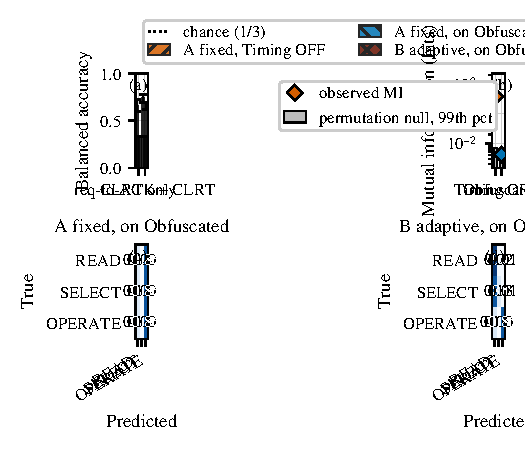
\includegraphics{figures/ndss/fig_leakage}
  \caption{Transaction-class leakage under the two attacker models, leaving out one grouped run at a time.
  (a) Balanced accuracy; whiskers span the 22 held-out runs and are not a confidence interval.
  (b) Mutual information against a within-run permutation null. (c) and (d) Row-normalized
  confusion using both intervals.}
  \label{fig:leakage}
\end{figure}

\textbf{Setup.} The features are the two separately measurable intervals; their sum, the total
response time, is excluded so that no feature is a linear combination of the others. Separately
measurable is not statistically independent and we do not assume it is: the classifier is given
both and may exploit any dependence between them, which is what the adaptive result below does. We
estimate mutual information for the CLRT in bits against a null built by shuffling class labels
within each grouped run over 1{,}000 permutations, preserving the per-run class counts. Every fold
leaves out one grouped run, and we report the spread of the 22 held-out-run scores as a range.

\textbf{RO3.} Consider first what the mechanism does to the two intervals before any classifier is
applied. Under Timing OFF the classes separate mainly along the post-acknowledgment axis, with
medians of 2.116, 2.050 and 2.937~ms for READ, SELECT and OPERATE against
request-to-acknowledgment medians of 0.555, 0.555 and 0.558~ms, which barely separate them at all.
Under the mechanism that axis collapses: all three medians sit at 4.000~ms and READ and SELECT
overlap. What remains is a horizontal offset, with the request-to-acknowledgment median moving to
21.336, 21.239 and 20.650~ms, because the read lane is timed from the outstation's acknowledgment
and the control lane from the request. The two intervals plotted against each other, which is how
that collapse and that offset look, are published with the artifact.

In Figure~\ref{fig:leakage}, we show the two attacker models.

The fixed adversary trained on
Timing OFF traffic reaches 0.652 balanced accuracy on held-out Timing OFF exchanges using the
CLRT alone, and 0.736 using both intervals. Applied unchanged to obfuscated traffic, it falls to
0.333 and 0.334, which is chance. Mutual information between the CLRT and the class falls from
0.383~bits to 0.004~bits; the Timing OFF value lies far above its permutation null at the
resolution of the test ($p = 0.001$ with 1{,}000 permutations), and the obfuscated value lies
inside its null ($p = 0.084$), so the test does not reject the hypothesis that the obfuscated
estimate is null noise. Failing to reject is not evidence of zero: with 1{,}000 permutations the
test resolves differences of this size only so far, and a small residual dependence would look the
same. For the evaluated fixed Random-Forest attacker, then, three-class transaction identification
falls to approximately chance, and no dependence between the cross-layer response time and the
class survives at the resolution of this test. Note that this holds for the two features we give it; the plaintext function code is
outside a timing-only feature set and still names the operation. 

The adaptive adversary gives two results, and they answer different questions. Retrained on
obfuscated traffic it stays at chance, 0.333, on the CLRT alone: the targeted feature is
suppressed against a retrained adversary and not only against a fixed one. The same adversary
recovers to 0.651 when it is given both intervals, because the read and control paths are timed
from different events, so their acknowledgment latencies differ. The confusion panels show the
shape of that recovery, with OPERATE separable while SELECT stays confused with READ.

We state the cost of that difference rather than leave it to be inferred. On the
request-to-acknowledgment interval alone, balanced accuracy rises from 0.380 under Timing OFF to
0.662 under the mechanism: almost nothing about the class before the mechanism runs, and the most
informative single feature afterwards. The mechanism does not merely fail to remove that feature,
it creates it, because holding the acknowledgment for $D_A$ displaces an interval the two lanes
compute from different events. Against an adversary using both intervals and allowed to retrain,
the net effect is a fall from 0.736 to 0.651, or 0.085 on a three-class problem whose chance is
0.333.

The targeted feature is therefore suppressed under both conditions, the cross-layer response time
alone leaving fixed and retrained adversaries alike at 0.333. What retraining recovers, it
recovers from the request-to-acknowledgment interval, which the mechanism does not target and does
make more informative, and that residual bounds the result. Formby et
al.~\cite{formbyWhosControlYour2016} profile devices from undefended traffic, which motivates the
fixed condition; their setting does not restrict an observer of this mechanism to an unchanged
model, and we do not read it as doing so. One way to close the residual is to time both paths
from the same event, which we leave to future work. We do not claim it is the only way: we have
not searched the space of defenses that might close it differently.

\subsection{Limitations}
\label{sec:eval:limits}

Each limitation below bounds one of the results above, and we name which.

\textbf{One Device, One Campaign.} The evidence is one SEL-751A behind one Tofino-1 in one
five-hour campaign, and the runs are grouped collections rather than independent replications, so
every result from RO1 to RO5 is a statement about this device and this window and every spread is
within-campaign variability.

\textbf{What RO3 Establishes.} RO3 characterizes the Random-Forest attacker we evaluated rather
than every classifier, and the adaptive adversary recovers 0.651 balanced accuracy from the
difference between the two events, which is the bound on what it achieves.

\textbf{What RO2 Rests On.} Only the master-facing link was captured, so the realized
per-transaction hold $J$ and the relay-facing release at $T_0 + J$ are configured rather than
observed: RO2 is a claim about the interval the master sees and reports no result per $J$.

\textbf{What RO4 Observes.} The admission horizon $H$ is computed in the control plane rather than
enforced by the data plane, so the saturation at 31.07~ms is an observed transition and not a proof
that the two coincide, and the sweep offsets likewise come from the configuration table rather
than a per-point readback.

\textbf{The Residual Is Not Attributed.} The switch's own release instants were not captured, and
the program cannot supply them: the timestamp registers it declares are never written. What the
measured distribution shows around the configured value is therefore a net difference between two
releases, not a delay we can place inside the switch.

On a separately instrumented build that adds two registers per lane, keyed on the outcome marking
a blocker that terminates because its deadline passed, the medians over twelve transactions are
1{,}706~ns on the acknowledgment lane and 1{,}705~ns on the response lane, with standard
deviations of 8.7 and 8.0~ns, about $4\times10^{-4}$ of the 4~ms configured interval. The first
blocker's ingress timestamp follows the deadline by a median of 12.5 and 13.5~ns, bounding when a
blocker first observed the expiry rather than when the release decision was taken, which the
program does not timestamp.

Four limits apply, and the first is why we do not simply call it $\varepsilon$. Both timestamps
are taken in ingress on a recirculating blocker token, so the interval ends at the last blocking
action and not at the wire, and this program carries no egress timestamp. We report an internal
blocker-termination interval and do not claim it bounds $\varepsilon$ in either direction, because
the blocker's last traffic-manager service precedes its return to ingress and the ordering of the
two endpoints is not established. It comes from a \emph{different build} than the campaign, so it
characterizes the mechanism rather than any exchange in the measured distributions; that build is
identified by the recorded patch over the frozen program, with the build tree, its loader
configuration and the loader's log agreeing on which binary ran. Twelve transactions at one
configuration are not a drain bound over load. Comparing the instrumented build against the frozen
one over 200 polls each gives mean cross-layer response times of 4.000282 and 3.999470~ms with
sample standard deviations of 0.0153~ms in each: one pair of captures at one configuration, which
does not establish equivalence, and which would not reveal equal movement in both releases.

\textbf{What RO5 Counts.} The overhead of RO5 is measured on the master-facing link, where the
switch's internal blocker traffic never appears. The zero-retransmission result is bounded the
same way: because the program suppresses a response retransmission that matches an already-seen
transport position while its transaction is live, such a copy would be absorbed inside the switch
and would not reach a master-facing capture.

We probed that suppression. A response lost downstream of the switch is recovered by exactly such
a retransmission, so a mechanism that discarded it would break loss recovery. Dropping the
response inbound at the master, scoped to one connection, leaves it unacknowledged and the
outstation retransmits on its own timer; three further copies crossed the switch and reached the
master's interface, at 3.20, 9.21 and 20.25~s, every one forwarded rather than absorbed.

The probe does not show that duplicate suppression preserves loss recovery. The filter dropped
every copy for the whole test rather than only the original, so nothing was acknowledged and the
application recovered nothing, and the capture is taken ahead of the filter, so it records arrival
at the interface. The copies also arrived long after the transaction had retired, the first
2.97~s after a transaction live for about 24~ms, so they met the path a stale token takes rather
than the path a duplicate of a live transaction takes, which is the case the concern is about.
Reaching that path needs an outstation whose retransmission timer is of the same order as the
hold; on this relay it is about three orders larger. The mechanism forwards late copies, and the
live-window case stays open.

\textbf{A Lost OPERATE Cannot Be Repaired.} The control lane has a second and worse case, which we
found by reading the program rather than by measuring it. After the switch releases an OPERATE
toward the relay it keeps that command's application generation as a spent marker, and clears it
only when the next SELECT arrives. A later OPERATE carrying the same generation is classified a
duplicate and dropped. If the released command is lost on the relay-facing link, the master's
transport repairs the loss by retransmitting exactly those bytes, with the same generation, and
the switch discards the packet the repair depends on. Forwarding a command out of the switch is
not delivery to the relay, and the program cannot tell the two apart because the relay-facing link
is not instrumented. No capture in this work exercises the path: the campaign's 5{,}280 OPERATE
exchanges lost nothing and every control operation returned success, which is the normal case
working rather than evidence that the failure case is handled. We therefore claim no loss recovery
on the control path, and exactly-once execution is neither provided nor claimed.

\textbf{The Tail Is Not Eliminated.} A fixed read-path release budget leaves about one exchange
in a thousand answering too late to be scheduled, and a comparable fraction of protected READ
exchanges more than 1~ms from the configured value. RO1 is a claim about the distribution, not about every transaction in
it.
